\section{Introduction}
\label{sec:introduction}

% state the learning objective 
The objective of this laboratory assignment is to design an AC/DC converter circuit, that receives an AC voltage of 230V and 50Hz ($v_{in}(t)$) and outputs a DC voltage of 12V. In order to achieve the goal, it was possible to choose the winding ratio of the transformer, and the architecture of the Envelope Detector and Voltage Regulator circuits. A \textit{Merit} score is obtained as a function of the chosen architecture's cost and how accurate the output is (relative to the aimed 12V DC output). 

The chosen circuit is presented in Figure \ref{fig:circ}


\begin{figure}[h] \centering
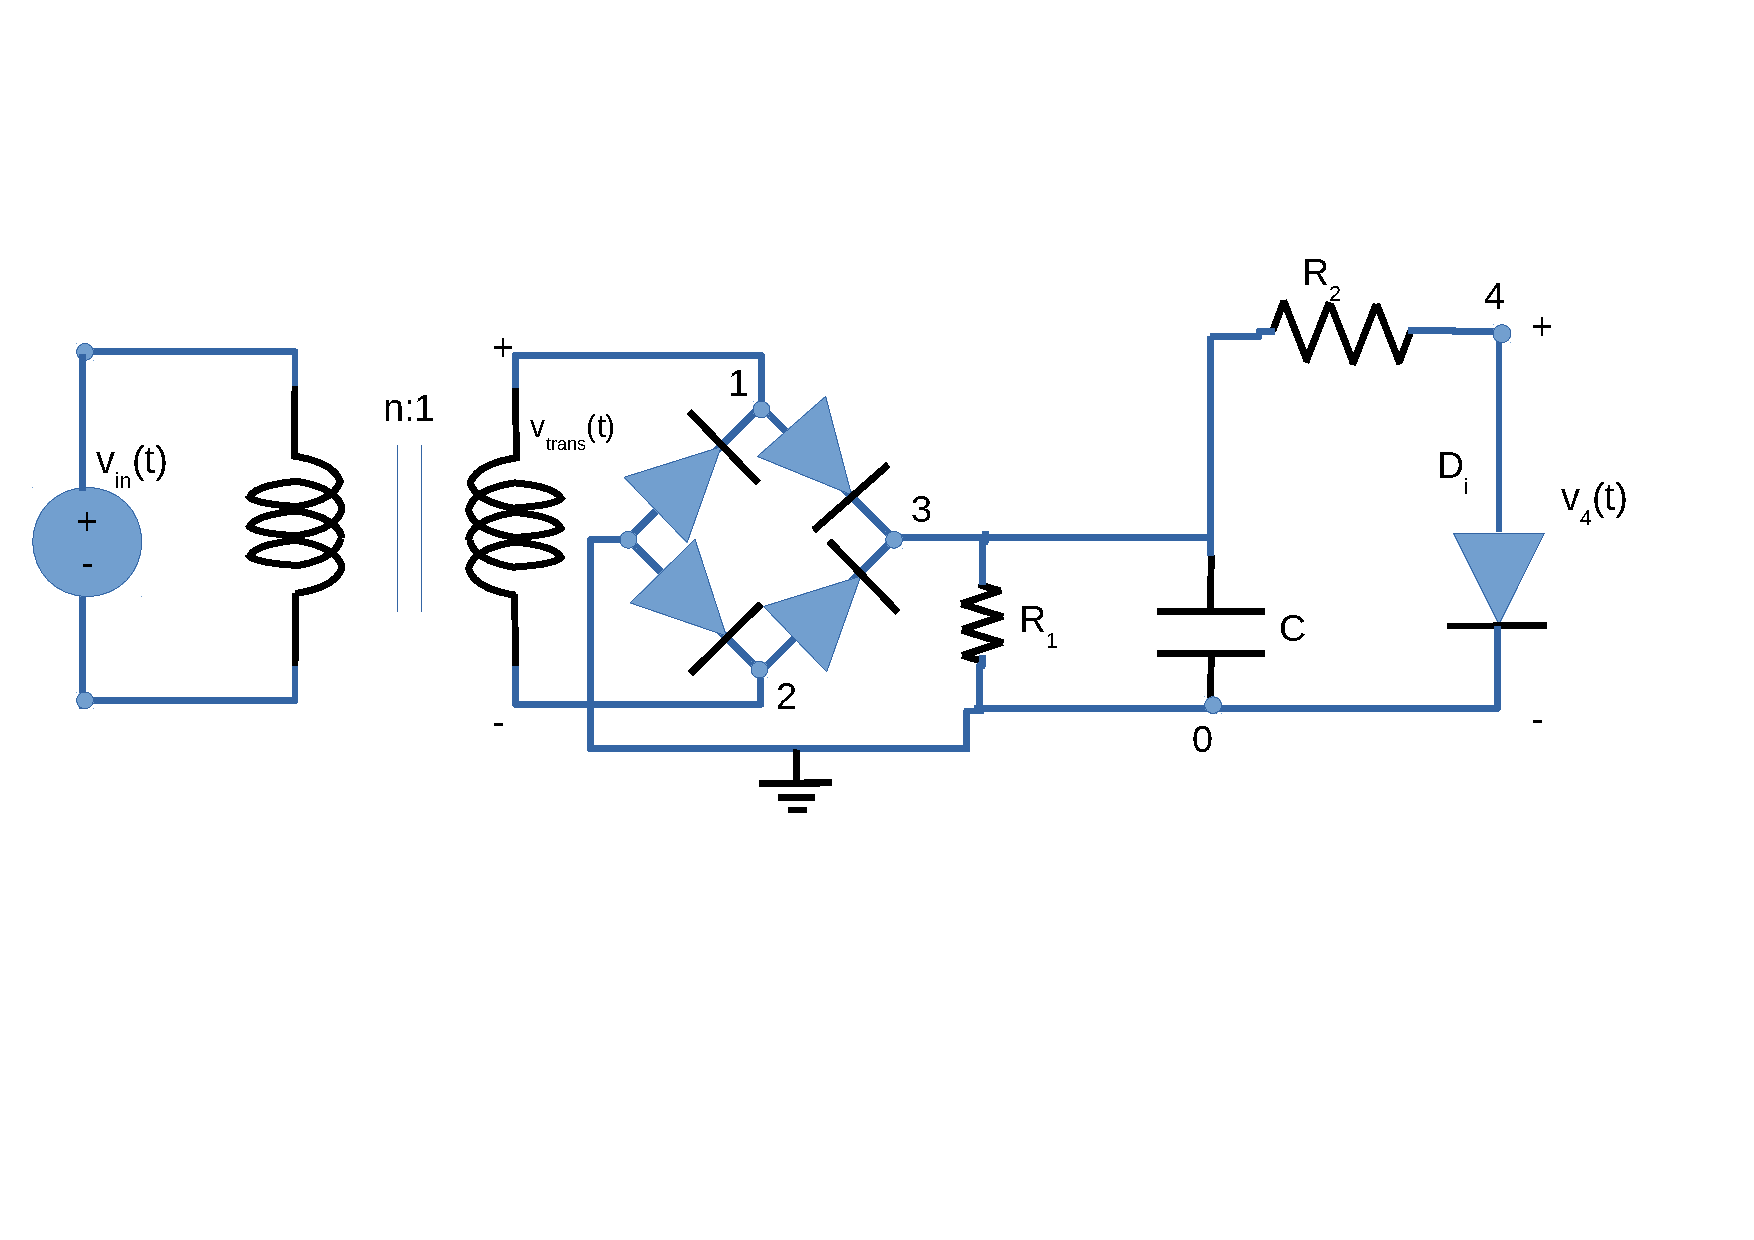
\includegraphics[width=0.9\linewidth]{circ.pdf}
\caption{AC/DC Converter Circuit.}
\label{fig:circ}
\end{figure}

in which $R_1 = 20000 \si{\ohm}$, $C=0.00001 F$, $R_2 = 2000 \si{\ohm}$, $n=17$, $D_i$ is a set of 17 diodes (whose parameters will be described in the following sections), and the numerical values next to the tiny circles specify the number of the nodes. The diamond of four diodes will also be described later on.


In Section~\ref{sec:analysis}, using \textit{Octave}, a theoretical analysis is presented, in which we describe the theoretical model used to the predict the output of the Envelope Detector and Voltage Regulator circuits and the results of the described analysis are presented. In this Section's last subsection (Subsection \ref{subsec:theo_merit}), the cost of the circuit and Merit score are determined. In Section~\ref{sec:simulation}, the circuit is analyzed by simulation, but using the Ngspice software, instead of a chosen theoretical model. The results are compared in Subsection~\ref{subsec:compare} (the last of this third Section). The conclusions of this study are outlined in Section~\ref{sec:conclusion}.